\section{Vermittlung}

\paragraph{Leitungsvermittlung}
\begin{items}
  \item Verbindung ist \emph{durchgehender Kanal} mit konstanter Bandbreite für exklusive Nutzung
  \item \textbf{Multiplexing}: \emph{starres Multiplexing} möglich \\*
    - \emph{Frequenzmultiplex}: Feste Zuweisung eines Frequenzabschnitt im Frequenzband \\*
    - \emph{Zeitmultiplex}: Feste Zuweisung eines Zeitschlitz (\emph{time slot}) in jedem Frame
  \item \textbf{Eigenschaften}: \\*
    - Aufbau eines durchgehenden Übertragungskanals zwischen Endsystemen \\*
    - Zwischensysteme: Zustandshaltung statt Adressinformation nötig \\*
    - zugesicherte, feste Datenrate \( \leadsto \) ungenutzte Ressourcen bei Nichtverwendung \\*
    - Übertragungsverzögerungen nur physikalisch bedingt \\* \phantom{-} \phantom{-} \( \leadsto \) keine Schwankungen durch Puffer \\*
    - Reihenfolgentreue Bitfolgenübertragung
  \item \textbf{Einsatzgebiete}: Telefonnetze, GSM
\end{items}

\paragraph{Paketvermittlung}
\begin{items}
  \item \textbf{Prinzip}: Weiterleitung anhand von Kontrollinformation in Paket \\*
    (Zieladresse in Datagrammen, lokale Kennung bei virtuellen Verbindungen)
    \item Zwischensysteme Speichern Pakete in \emph{Warteschlangen} \( \leadsto \) Paketverlust möglich\\*
    	Variable Verzögerungszeiten
   \item Üblicherweise Zeitmultiplex (keine Reservierung von Ressourcen)
  \item \textbf{Varianten}: \\*
    - \emph{verbindungslos}: Datagramme \\*
    - \emph{verbindungsorientiert}: virtuelle Verbindungen
\end{items}
\begin{figure}[H]\centering\label{Paketvermittlung}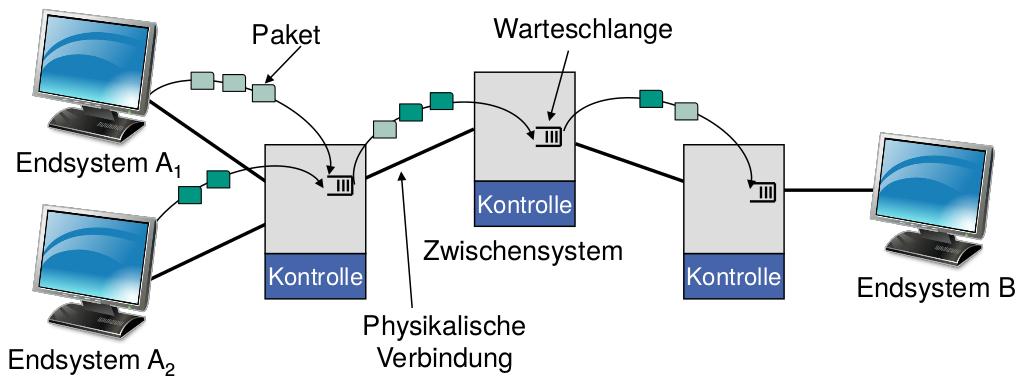
\includegraphics[width=0.33\textwidth]{Paketvermittlung}\end{figure}

\paragraph{Paketvermittlung --- Datagramme}
\begin{items}
  \item Pakete (= Datagramme) werden als isolierte Einheiten betrachtet
  \item \textbf{Zieladresse} in jedem Datagramm enthalten \( \leadsto \) keine Verbindungsverwaltung nötig
  \item \textbf{Routing}: Pakete können verschiedene Wege im Netz nehmen \\*
    \( \leadsto \) Datagramme können bei Empfänger unsortiert ankommen
\end{items}

\paragraph{Paketvermittlung --- virtuelle Verbindungen}
\begin{items}
  \item Fester Übertragungsweg zwischen zwei Endsystemen
  \item \textbf{Reihenfolgetreue}: Alle Pakete nehmen den selben Weg
  \item \textbf{Kennung}: \emph{virtual circuit identifier} (VCI) für jeden Übertragungsabschnitt
  \item \textbf{Zieladresse} nur bei Aufbau nötig, Vermittlungsinformationen in Zwischensystemen
  \item \textbf{Ablauf}: Verbindungsaufbau \( \to \) Datenübertragung \( \to \) Verbindungsabbau
\end{items}

\paragraph{Nachrichtenvermittlung}
\begin{items}
  \item \emph{Vermittlung von Anwendungsnachrichten}
  \item Vermittlung üblicherweise mittels mehrerer Pakete \\*
    \( \leadsto \) \emph{Segmentierung} und \emph{Reassemblierung} in Zwischensystemen (alle Teile müssen jeweils an gleiches System weitergeleitet werden)
  \item \( \leadsto \) \emph{Ende-zu-Ende-Verzögerung wesentlich höher als bei Paketvermittlung}
\end{items}

\paragraph{Vermittlungsschicht --- Überblick}
\begin{items}
  \item \textbf{Ende-zu-Ende}: transportiert Segmente zwischen Endsystemen
  \item Sender: Kapselt Segmente in Datagramme
  \item Empfänger: Segmente werden an Transportschicht ausgeliefert
  \item Protokolle in \emph{allen} Endsystemen und Routern
  \item \textbf{Router} werten Felder im Kopf aller Datagramme aus, die sie passieren
\end{items}

\paragraph{Forwarding und Routing}
\begin{items}
  \item \textbf{Forwarding} (\emph{Weiterleitung}): Datenebene \\*
    - Pakete werden von Eingang an passenden Ausgang (Tabelle) weitergeleitet\\*
    - Funktionen lokal in Router
    \smallskip
  \item \textbf{Routing} (\emph{Wegewahl}): Kontrollebene \\*
    - Ermittelt Wege für Pakete und darauf basierend Weiterleitungstabelle \\*
    - Betrachtet gesamtes Netz, benötigt Routingalgorithmus und -protokoll\\*
    - \emph{Konzepte}: \\
    \phantom{-} \( \cdot \) traditionell: in jedem Router implementiert, interagieren auf Kontrollebene \\*
    \phantom{-} \( \cdot \) \emph{software defined networking} (SDN): in logisch zentralen Servern implementiert
\end{items}

\paragraph{Vermittlungsschicht --- Begriffe}
\begin{items}
  \item \textbf{Router}: Auf Vermittlungsschicht operierendes Zwischensystem \\*
    - leitet Datagramme mithilfe von Weiterleitungstabelle weiter \\*
    - tauscht über Routingprotokolle Informationen mit anderen Routern aus
  \item \textbf{Route}: Weg eines Datagramms: Sequenz von Routern zwischen zwei Endsystemen
  \item \textbf{Link}: Übertragungsabschnitt zwischen 2 Routern (kann z.B. auch Brücken enthalten)
  \item \textbf{Port}: Eingangs-/Ausgangs-Netzwerkschnittstelle
\end{items}

\paragraph{Vermittlungsschicht --- Protokolle}
\begin{items}
  \item \textbf{IP} (\emph{internet protocol}): \\*
    unzuverlässige Datagrammübertragung
  \item \textbf{ICMP} (\emph{internet control message protocol}): \\*
    Kontrollinformationsaustausch innerhalb der Vermittlungsschicht
  \item \textbf{ARP} (\emph{address resolution protocol}): \\*
    Zuordnung von IP-Adressen zu Adressen der Sicherungsschicht
  \item \textbf{RARP} \emph{reverse ARP}: \\*
    Umkehrfunktionen von ARP
  \item \textbf{BGP} (\emph{border gateway protocol}), \textbf{RIP} (\emph{routing information protocol}), \textbf{OSPF} (\emph{open shortest path first}): Routingprotokolle
\end{items}

\paragraph{Vermittlung --- IP (Internet Protocol)}
\begin{items}
	\item Verbindungsloser, unzuverlässiger Vermittlungsdienst\\*
	 	(kein Kontext in Zwischen- oder Endsystemen)
  \item IP macht die ganze Vermittlung \( \leadsto \) nur ein einziges Vermittlungsprotokoll \\*
    - Interoperabilität erhöhen: Anzahl unterschiedlicher Interfaces verringern \\*
    - Kleinster gemeinsamer Nenner: Anzahl nutzbarer Netze maximieren
\end{items}
\begin{figure}[H]\centering\label{IP}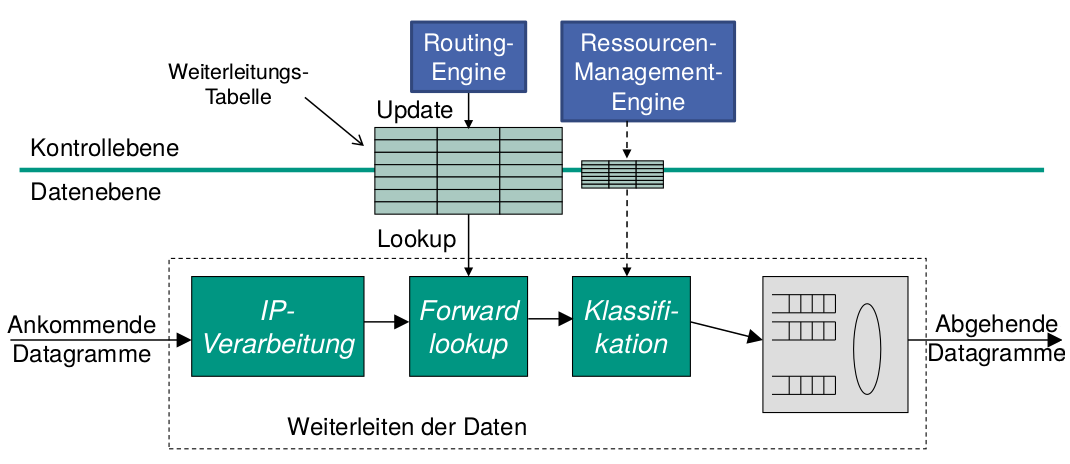
\includegraphics[width=0.4\textwidth]{IP}\end{figure}
\begin{figure}[H]\centering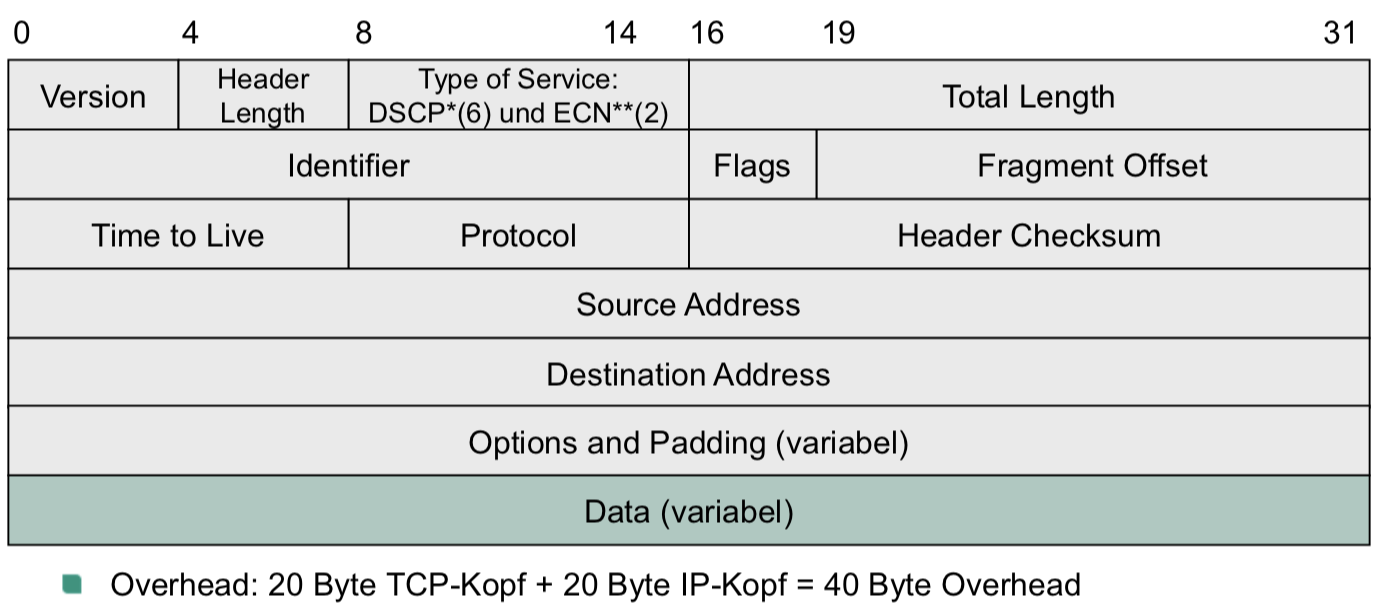
\includegraphics[width=0.4\textwidth]{IP4Header}\end{figure}

\paragraph{IP --- Fragementieren + Reassemblieren}
\begin{items}
  \item Anpassung an Maximallänge unterliegender Netze (\textbf{MTU}: \emph{maximum transfer unit})
  \item Fragmentieren überall möglich, Reassemblieren nur in Endsystem
  \item \textbf{Fragment-Offset} (Einheit: 8 Bytes) + Flag-Felder im IP-Kopf %\\*
%    - \emph{Bit 0}: reserviert, muss 0 sein \\*
%    - \emph{Bit 1}: 0 = darf fragmentiert werden, 1 = nicht \\*
%    - \emph{Bit 2}: 0 = letztes Fragment, 1 = nicht
\end{items}

\paragraph{IP --- Weiterleitung}
\begin{items}
  \item \textbf{Endsystem}: \\*
    - Rechner mit Zieladresse direkt verbunden \( \to \) Datagramm direkt zustellen \\*
    - Sonst: Datagramm-Übergabe an Standardrouter
    \smallskip
  \item \textbf{Weiterleitungstabelle}: Für jede Zieladresse (Endsystem- oder Netzadresse) \\*
    - \emph{Next-Hop-Router} (falls nicht im gleichen Netz) \\*
    - \emph{Netzschnittstelle}, an die Paket weitergeleitet wird \\*
    	(Schnittstelle, an der Next-Hop bzw. Endsystem hängt)\\*
    - Flags
\end{items}

\paragraph{IP --- Empfangsprozess}
\begin{items}
  \item \textbf{Überprüfungen}: \\* 
    - \emph{Kopflänge}, \emph{Datagrammlänge}, \emph{Prüfsumme} \\*
    - \emph{Versionsnummer} IP, \emph{Protokoll-Identifikation} \\*
    - \emph{Lebenszeit}, \emph{Adressklassen}
    \smallskip
  \item \textbf{Fehlerfall}: Benachrichtigung ICMP (\emph{internet control message protocol}) --- möglicherweise wird ICMP-Paket ausgesendet
\end{items}

\paragraph{IP --- Adressierung}
\begin{items}
  \item \textbf{Ziel}: Eindeutige Identifizierung aller Interfaces von Routern/Endsystemen
  \item \textbf{IP-Adressen}: Adressen der Vermittlungsschicht -- Kennung für Interfaces \\*
    - \emph{IPv4}: 32 Bit (z.B. 207.142.131.235) \\*
    - \emph{IPv6}: 128 Bit (z.B. 2001:0db8:85a3:08d3:1319:8a2e:0370:7344)
    
    \medskip
  \item IP-Adresse unterteilt in \\*
    - \emph{Subnetz-Teil}: high order bits \\*
    - \emph{Endsystem-Teil}: low order bits
  \item \textbf{Subnetz}: Interfaces mit selbem Subnetz-Teil, können ohne Router kommunizieren
  \item \textbf{CIDR} (Classless Inter-Domain Routing): Subnetz-Teil kann unterschiedlich lang sein\\*
  	Format: a.b.c.d/x (x: Anzahl Bits im Subnetz-Teil, z.B. 200.23.16.0/24)
\end{items}

\paragraph{Adresszuteilung}
\begin{items}
	\item \textbf{Provider}: Erhält Block von \textbf{ICANN} (\emph{internet corporation for assigned names/numbers}) \\*
	Allokiert IP-Adressen, verwaltet DNS, weist Domainnamen zu
	\item Netz bekommt Subnetz-Teil von seinem Provider zugeordnet
  \item \textbf{Manuell}: Durch Systemadministrator
  \item \textbf{Dynamisch}: DHCP-Server liefert auf Anfrage IP-Adresse für Client
\end{items}

\paragraph{DHCP (dynamic host configuration protocol)}
\begin{items}
	\item Dynamischer Bezug von IP-Adressen durch Endsysteme
	\item Beschränkte zeitliche Gültigkeit (\emph{lease})
	\item Zusätzlich Subnetzmaske, Adresse des Default-Gateways, DNS-Server, \dots möglich
	\item \textbf{Ablauf}: [Discover, Offer], Request, Ack (jeweils als Broadcast)
\end{items}

\paragraph{Internet Control Message Protocol (ICMP)}
\begin{items}
  \item Einzelne Datagrammverluste meldet IP nicht (unzuverlässiger Dienst)
  \item Schwerwiegende Probleme (z.B. Leitungsunterbrechung): Mitteilung via ICMP
  \item \( \Rightarrow \) ICMP tauscht Fehlernachrichten, Statusanfragen und Zustandsinformationen aus
  \medskip
  \item \textbf{Echo} + Antwort (\emph{echo and echo reply}): \\*
    - Aktivitätsüberprüfung von Kommunikationssystemen \\*
    - Empfänger von Echo-Anfrage sendet erhaltene Daten in Echo-Antwort zurück
  \item \textbf{Zeitstempel} + Antwort (\emph{timestamp and timestamp reply}): \\*
    - Bestimmung von Umlaufzeiten (\emph{round trip time}, RTT)
\end{items}

\paragraph{IPv6}
\begin{items}
  \item \textbf{Problem}: Adressraum von IPv4 geht aus \( \Rightarrow \) Erhöhung Adresslänge von 32 auf 128 Bit 
  \item Optimiere \textbf{Format des Headers} für schnelle Verarbeitung:\\*
    - feste Kopflänge (40 Byte), Optionen als Erweiterungsköpfe (\emph{next header}) \\*
    - keine Unterstützung von Fragmentierung, keine Prüfsumme
   \item ICMPv6: neue Version von ICMP
    \begin{figure}[H]\centering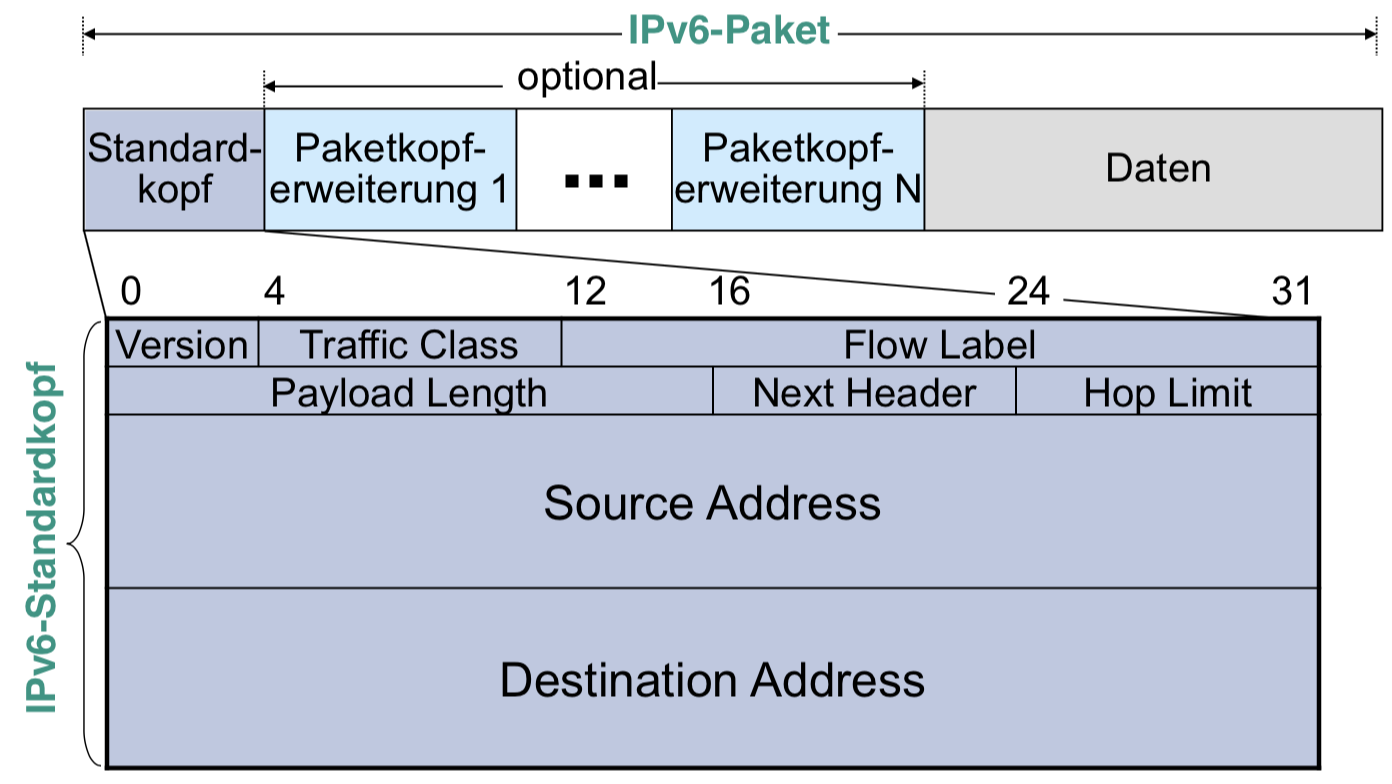
\includegraphics[width=0.4\textwidth]{IP6Header}\end{figure}
\end{items}

\paragraph{Routing --- Prinzipien}
\begin{items}
  \item Ziel: Guten Weg durch Netz finden (geringste Kosten)
  \item \textbf{Netzgraph}: Netz wird als Graph verstanden \\*
    - \emph{Knoten}: Router \\*
    - \emph{Kanten}: Übertragungsabschnitte (Kantenkosten z.B. Verzögerung, Preis,\dots)
  \item \textbf{Pfad}: Folge von Knoten (meist Pfad mit kürzester Länge gesucht)
\end{items}

\paragraph{Routing-Verfahren --- Dynamik}
\begin{items}
  \item \textbf{Nicht adaptiv}: Routen ändern sich sehr selten, wesentlich seltener als Verkehr
  \item \textbf{Adaptiv}: Routen ändern sich abhängig von Verkehr und Topologie \\*
    - Routenänderungen periodisch oder reaktiv \\*
    - \emph{Zielkonflikt}: Systeme haben ggf kein Live-Abbild des Netzes \\*
      \phantom{-} \phantom{\( \cdot \)} ggf hohe Netzbelastung durch Routing-Informationsaustausch
\end{items}

\paragraph{Routing-Verfahren --- statisches Routing}
\begin{items}
  \item \textbf{Beispiel}: Abhängig von Zufallszahl weiterleiten nach B, C oder D
\end{items}

\paragraph{Routing-Verfahren --- zentralisiert}
\begin{items}
  \item Adaptives Verfahren
  \item \textbf{Routing Control Center}: Für Berechnung/Verteilung der optimalen Pfade \\*
    - Systeme senden periodisch Zustand an RCC \\* \phantom{-} \phantom{\( \cdot \)} (aktive Nachbarn, Warteschlangenlängen,\dots)
  \item \textbf{Vorteile}: \\*
    - RCC hat alle Informationen \( \leadsto \) kann perfekte Entscheidungen treffen \\*
    - Systeme müssen kein Routing betreiben
  \item \textbf{Nachteile}: \\*
    - Berechnungsdauer für große Netze ggf sehr lang \\*
    - Ausfall RCC lähmt ganzes Netz \\*
    - Inkonsistenzen möglich, da Systeme nah an RCC Tabellen schneller erhalten \\*
    - starke Belastung des RCC
\end{items}

\paragraph{Routing-Verfahren --- isoliert}
\begin{items}
  \item \textbf{Prinzip}: Jedes System entscheidet nur anhand eigener Informationen
   \item kein Austausch von Routinginformationen zwischen Systemen

    \medskip
  \item \textbf{Fluten}: Jedes eingehende Datagramm auf jeder Übertragungsleitung weiterleiten
  \item \emph{Fluteindämmung}: \\*
    - \emph{Sequenznummern} für Duplikaterkennung \\*
    - \emph{Lebensdauerkontrolle} durch Zählen der Übertragungsabschnitte (\emph{hops})
  \item \emph{Varianten}: \\*
    - \emph{selektives Fluten}: Weiterleitung nicht auf allen Übertragungsabschnitten \\*
    - \emph{random walk}: Zufällige Auswahl eines Übertragungsabschnittes

	\medskip
  \item \textbf{Hot Potato}: JDatagramme so schnell wie möglich weiterleiten \\*
    \( \leadsto \) Übertragungsabschnitt mit kürzester Warteschlange wählen
  \item \emph{Varianten}: \\*
    - nie an Herkunftsleitung weiterleiten \\*
    - Kombination mit statischem Routing: statisches Verfahren zur Auswahl von \\* \phantom{-} \phantom{\( \cdot \)} Leitung mit Warteschlangenlänge unter Schwellwert
\end{items}

\paragraph{Routing-Verfahren --- Verteiltes adaptives Routing}
\begin{items}
  \item \textbf{Prinzip}: Systeme tauschen Routing-Informationen mit Nachbarn aus \\*
    - jedes System unterhält Routing-Tabelle
  \item \textbf{Varianten}: \\*
    - periodischer Informationsaustausch \\*
    - Austausch nur bei größeren Änderungen
\end{items}

\paragraph{Routing-Algorithmen --- Übersicht}
\begin{items}
  \item \textbf{Distanz-Vektor-Algorithmen}: \\*
  	- Distanz als Routing-Metrik \\*
    - jeder Router kennt Distanz zu allen anderen Systemen im Netz \\*
    - dazu Austausch der Distanzen zwischen Nachbarn\\*
    - \emph{Problem}: kürzerer langsamer Weg wird längerem schnelleren vorgezogen
  \item \textbf{Link-State-Algorithmen}: \\*
  	- Unterschiedliche Routing-Metriken \\*
    - berücksichtigt aktuelle Zustände der Netzanschlüsse \\*
    - jeder Router kennt und nutzt ganze Netztopologie zur Berechnung \\*
\end{items}

\paragraph{Link-State vs. Distanz-Vektor}
\begin{items}
	\item \textbf{Komplexität Kontroll-Pakete}: \\*
	- \emph{Link-State}: jedes System muss Kosten aller Links kennen, Änderungen müssen an \\* \phantom{-} \phantom{\( \cdot \)} alle Systeme geschickt werden \( \leadsto  O(nE) \) Pakete\\*
	- \emph{Distanz-Vektor}: Änderungen nur an benachbarte Systeme weitergegeben
	\item \textbf{Konvergenzgeschwindigkeit}: \\*
	- \emph{Link-State}: schnelle Konvergenz (\( O(n^2) \)),  schleifenfrei, Oszillationen möglich \\*
	- \emph{Distanz-Vektor}: langsame Konvergenz, Schleifen sowie Count-to-Infinity möglich
	\item \textbf{Robustheit}: \\*
	- \emph{Link-State}: Routenberechnungen separiert \( \leadsto \) Robustheit \\*
	- \emph{Distanz-Vektor}: ein System kann inkorrekte Pfade zu allen Zielen verbreiten
	\item \textbf{Fazit} \\*
	- \emph{Link-State}: Konvergiert schneller, ist robuster \\*
	- \emph{Distanz-Vektor}: einfacher zu implementieren
\end{items}

\paragraph{Routing-Algorithmen --- Distanz-Vektor}
\begin{items}
    \item \textbf{verteilt}: jeder Router erhält Infos von direkten Nachbarn, führt Berechnung durch und verteilt dann neue Informationen an direkte Nachbarn
    \item \textbf{iterativ}: Verteilen + Berechnen von Informationen so lange, bis keine Information mehr ausgetauscht wird

\end{items}

\paragraph{Distanz-Vektor --- Distanz-Vektor-Tabelle}
\begin{items}
	\item \textbf{Distanz-Vektor-Tabelle}: \\*
	- Grundlegende, in jedem System vorhandene Datenstruktur \\*
	- Zeilen für alle möglichen Ziele, Spalten für direkte Nachbarn \\*
  \item \textbf{Beispiel}: \( X \) will Daten über direkten Nachbar \( Z \) an \( Y \) weiterleiten \\*
    - \( D^X(Y,Z) = c(X,Z) + \underset{w}{\text{min}}\{ D^Z(Y,w) \} \)
  \item \textbf{Beispiel}: \( D^E(A,D) \) \\*
    - erster Übertragungsabschnitt: \( E \to D \) \\*
    - Tabelleneintrag: Kosten \( E \to D \) (2) + minimale Kosten \( D \to A \) (3)
\end{items}
\begin{figure}[H]\centering\label{DistanzVektor}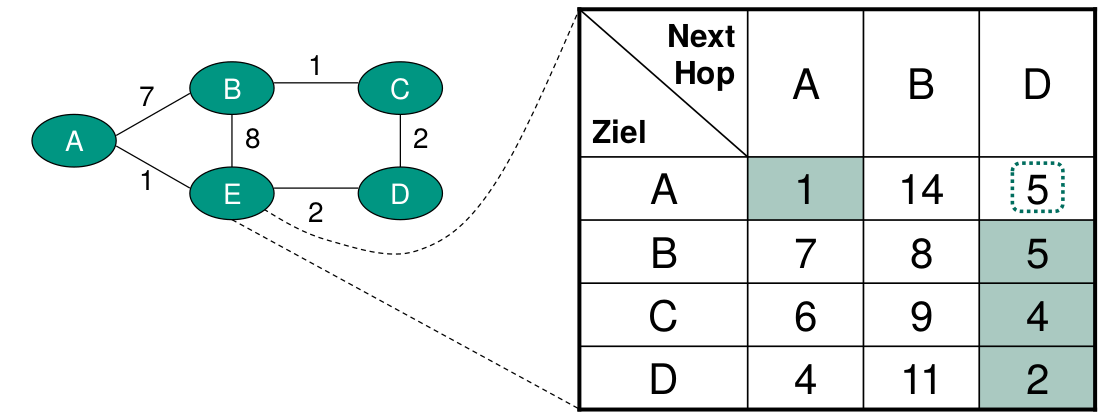
\includegraphics[width=0.4\textwidth]{DistanzVektor}\end{figure}

\paragraph{Distanz-Vektor --- Distanz-Vektor-Algorithmus (Bellman-Ford)}
\begin{items}
  \item \textbf{Initialisierung}: \\*
    - für alle Nachbarn \( v \): \( D^X(*,v) = \infty \), \( D^X(v,v) = c(X,v) \) \\*
    - für alle Ziele \( y \): sende \( \underset{w}{\text{min}}D^X(y,w) \) allen Nachbarn (\( w \) enthält alle Nachbarn)
  \item \textbf{Schleife}: \\*
    - geänderte Abschnittskosten: für alle Ziele \( y \): \( D^X(y,V) \coloneqq D^X(y,V) + d \) \\*
    - Update von Nachbarn: kürzester Pfad von \( V \) zu Ziel \( Y \) hat sich um \( \alpha \) geändert \\*
    \phantom{-} \( \leadsto \) \( D^X(Y,V) \coloneqq c(X,V) + \alpha \) \\*
    \phantom{-} \( \leadsto \) Falls neuer Minimalwert für ein Ziel \( Y \),  sende an alle direkten Nachbarn
  \item \textbf{Komplexität}: \( O(n^2k) \) für \( n \) Knoten und \( k \) Kanten
\end{items}

\paragraph{Distanz-Vektor --- Updateausbreitung}
\begin{items}
  \item \textbf{Good news}: schnelle Ausbreitung
  \item \textbf{Bad news}: langsame Ausbreitung, ggf Routing-Schleifen \\*
    \( \leadsto \) \textbf{Count to Infinity-Problem}
  \item \textbf{Poisoned Reverse}: Vermeidung von Routing-Schleifen, indem Routing-Information \( Y \) vorenthalten wird, wenn Weg über \( Y \) kürzer
\end{items}

\paragraph{Routing-Algorithmen --- Link-State-Routing}
\begin{items}
  \item \textbf{Prinzip}: Jedes System berechnet kürzeste Pfade durch gesamtes Netz\\*
    - Systeme müssen zu Beginn nur direkte Nachbarn kennen \\*
    - Entdecken von neuen Nachbarn zB mittels \code{HELLO}-Pakete \\*
    - \emph{link state broadcast}: Identität + Kosten zu Nachbarn werden allen Routern im Netz \\* \phantom{-} \phantom{\( \cdot \)} weitergeleitet (Fluten) \\*
    - Systeme lernen Topologie durch LSBs der anderen Systeme \\*
    - \emph{Ergebnis}: Alle Systeme haben \emph{identisches} Wissen über Netz
  \item \textbf{Implementierung}: Dijkstra-Algorithmus
\end{items}

\paragraph{software defined networking}
\begin{items}
  \item \textbf{Zentrale Eigenschaften}: \\*
    - Separierung von Kontroll- und Datenebene \\*
    - Flow-basierte Paketweiterleitung \\*
    - Logik an externen Controller ausgelagert \\*
    - Netzwerk programmierbar
  \item \textbf{Umsetzung}: \emph{open flow}-Protokoll (quasi-Standard, Alternativen existieren) \\*
    - regelt Kommunikation zwischen Controller und Switch \\*
\end{items}

\paragraph{Traditionelles IP-Routing}
\begin{items}
  \item Kontroll- und Datenebene in jedem Router
  \item \textbf{Vorteile}: \\*
    - Ausfallsicherheit (selbstorganisiert, verteilte Kontrolle, hohe Redundanz) \\*
    - Schnelle Reaktion (optimierte Routing-Hardware, lokale Routingentscheidung) \\*
    - Bewährtes Konzept
  \item \textbf{Nachteile}: \\*
    - proprietäre Management-Schnittstellen (Mischbetrieb schwierig) \\*
    - unflexibel (neue Funktionen hinzufügen schwierig, aufwändige Standardisierung) \\*
    - teuer (hochqualifiziertes Personal + Overprovisioning benötigt)
\end{items}
\begin{figure}[H]\centering\label{IPRoutingTraditionell}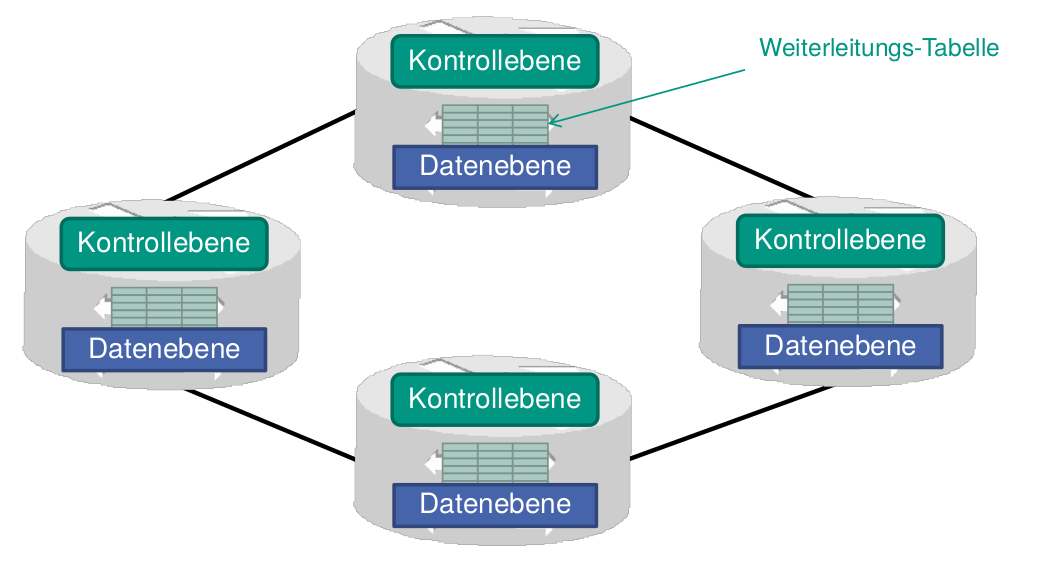
\includegraphics[width=0.33\textwidth]{IPRoutingTraditionell}\end{figure}

\paragraph{SDN-Routing}
\begin{items}
  \item \textbf{Vorteile}: \\*
    - logisch zentralisierte Sicht (Controller hat Netzüberblick, einfacher Einsatz von \\* \phantom{-} \phantom{\( \cdot \)} Graphenalgorithmen) \\*
    - neue Funktionalität in Software (als App im Controller, kürzere Entwicklungszeit) \\*
    - Trennung von Kontroll- und Datenebene (Innovationen unabhängig möglich, \\* \phantom{-} \phantom{\( \cdot \)} herstellerunabhängig durch offene Schnittstellen)
  \item \textbf{Nachteile}: \\*
    - Skalierbarkeit \\*
    - \emph{single point of failure} \\*
    - Kommunikation mit Controller langsam
\end{items}
\begin{figure}[H]\centering\label{SDNRouting}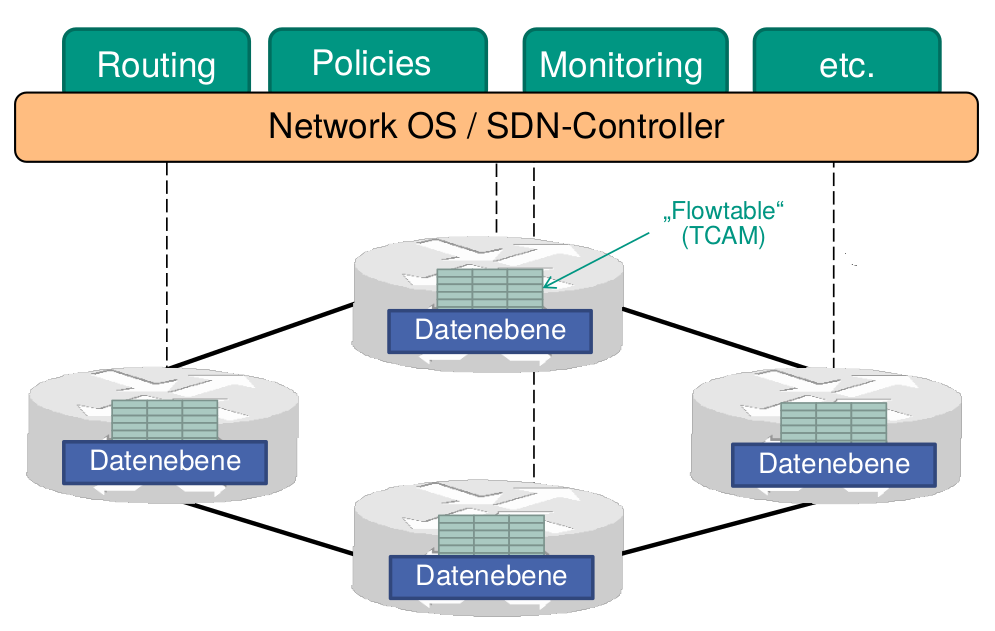
\includegraphics[width=0.33\textwidth]{SDNRouting}\end{figure}

\paragraph{SDN --- Paketweiterleitung}
\begin{items}
  \item \textbf{Traditioneller IP-Router}: \\*
    - kennt keine Flows \\*
    - Weiterleitung über Ziel-IP-Adresse (Longest Prefix Matching)
  \item \textbf{SDN-Switch}: \\*
    - Weiterleitung über Flowtable \\*
    - nutzt verschiedene IP-Kopf-Felder \\*
    - speichert Zustand pro Flow
\end{items}
\begin{figure}[H]\centering\label{SDNFlow}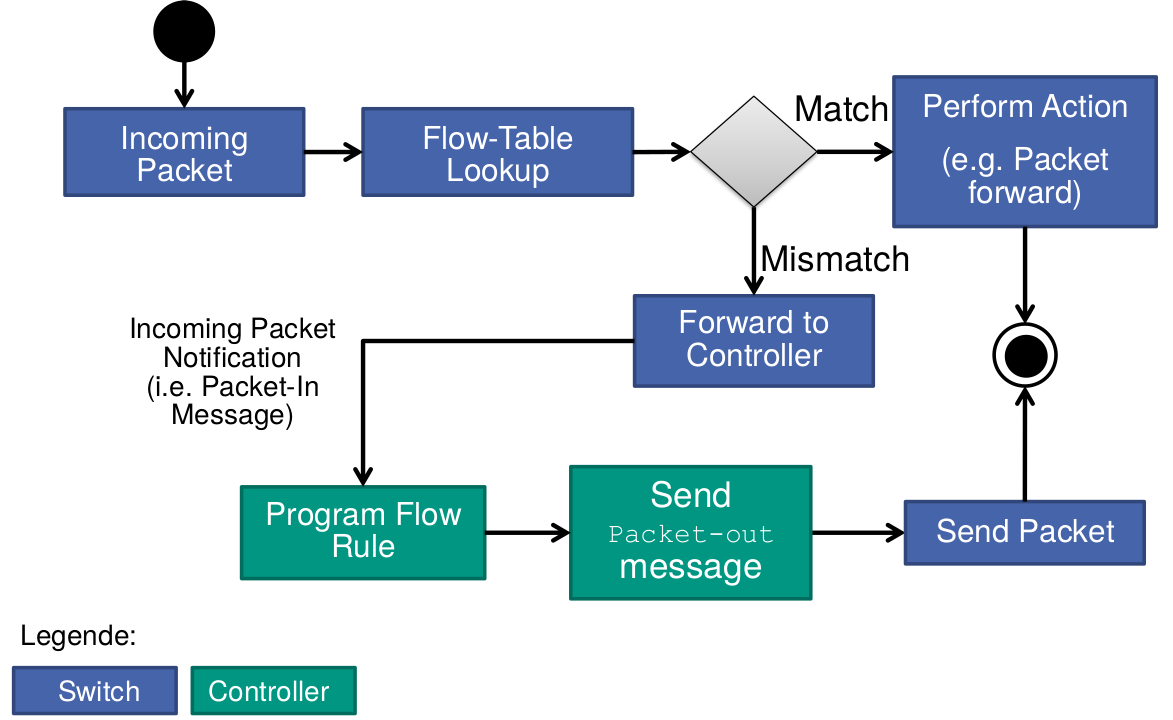
\includegraphics[width=0.45\textwidth]{SDNFlow}\end{figure}